\subsection{Đánh giá hiện thực Frontend}
\subsubsection{Đánh giá hiệu năng và tối ưu hóa}
Nhóm đã hoàn thành việc xây dựng giao diện người dùng (Frontend) cho toàn bộ các chức năng của hệ thống. Giao diện được thiết kế với mục tiêu thân thiện, dễ sử dụng và tương thích trên nhiều thiết bị khác nhau. 

Quá trình kiểm thử và đánh giá được thực hiện trực tiếp trên môi trường phát triển bằng các công cụ tiêu chuẩn công nghiệp: Google Lighthouse và Chrome DevTools. Để có cái nhìn khách quan về hiệu năng ứng dụng, nhóm thực hiện đo lường trên trang đại diện quan trọng nhất là Trang chủ (Home Page) - điểm tiếp cận đầu tiên của người dùng. Quá trình kiểm thử được thực hiện so sánh đối chứng giữa hai môi trường: Desktop (mạng ổn định) và Mobile (giả lập mạng 4G, CPU hạn chế).

\begin{table}[H]
    \centering
    \caption{So sánh hiệu năng Trang chủ: Desktop vs. Mobile}
    \label{tab:performance-comparison}
    \renewcommand{\arraystretch}{1.3} % Tăng khoảng cách giữa các dòng cho thoáng
    \begin{tabular}{|l|c|c|p{7cm}|}
        \hline
        \textbf{Tiêu chí} & \textbf{Desktop} & \textbf{Mobile} & \textbf{Phân tích chênh lệch} \\ \hline
        
        Performance & 
        95 & 
        60 & 
        Chênh lệch lớn do Mobile giả lập mạng chậm, tải ảnh chưa nén tốn thời gian. \\ \hline
        
        Accessibility & 100 & 97 & Tương đồng, cấu trúc HTML ngữ nghĩa tốt trên cả hai nền tảng. \\ \hline
        
        Best Practices & 100 & 100 & Mã nguồn bảo mật, không lỗi thư viện. \\ \hline
        
        SEO & 100 & 100 & Metadata được tối ưu hóa đầy đủ. \\ \hline
        
        \textbf{LCP (Tốc độ tải)} & 
        \textbf{0.8s} & 
        \textbf{3.2s} & 
        Mobile tải chậm hơn 4 lần do giới hạn băng thông giả lập (4G). \\ \hline
    \end{tabular}
\end{table}
\begin{figure}[H]
    \centering
    \begin{minipage}{0.48\textwidth}
        \centering
        % LƯU Ý: Đã đổi tên folder thành 8_Implement (không dấu cách)
        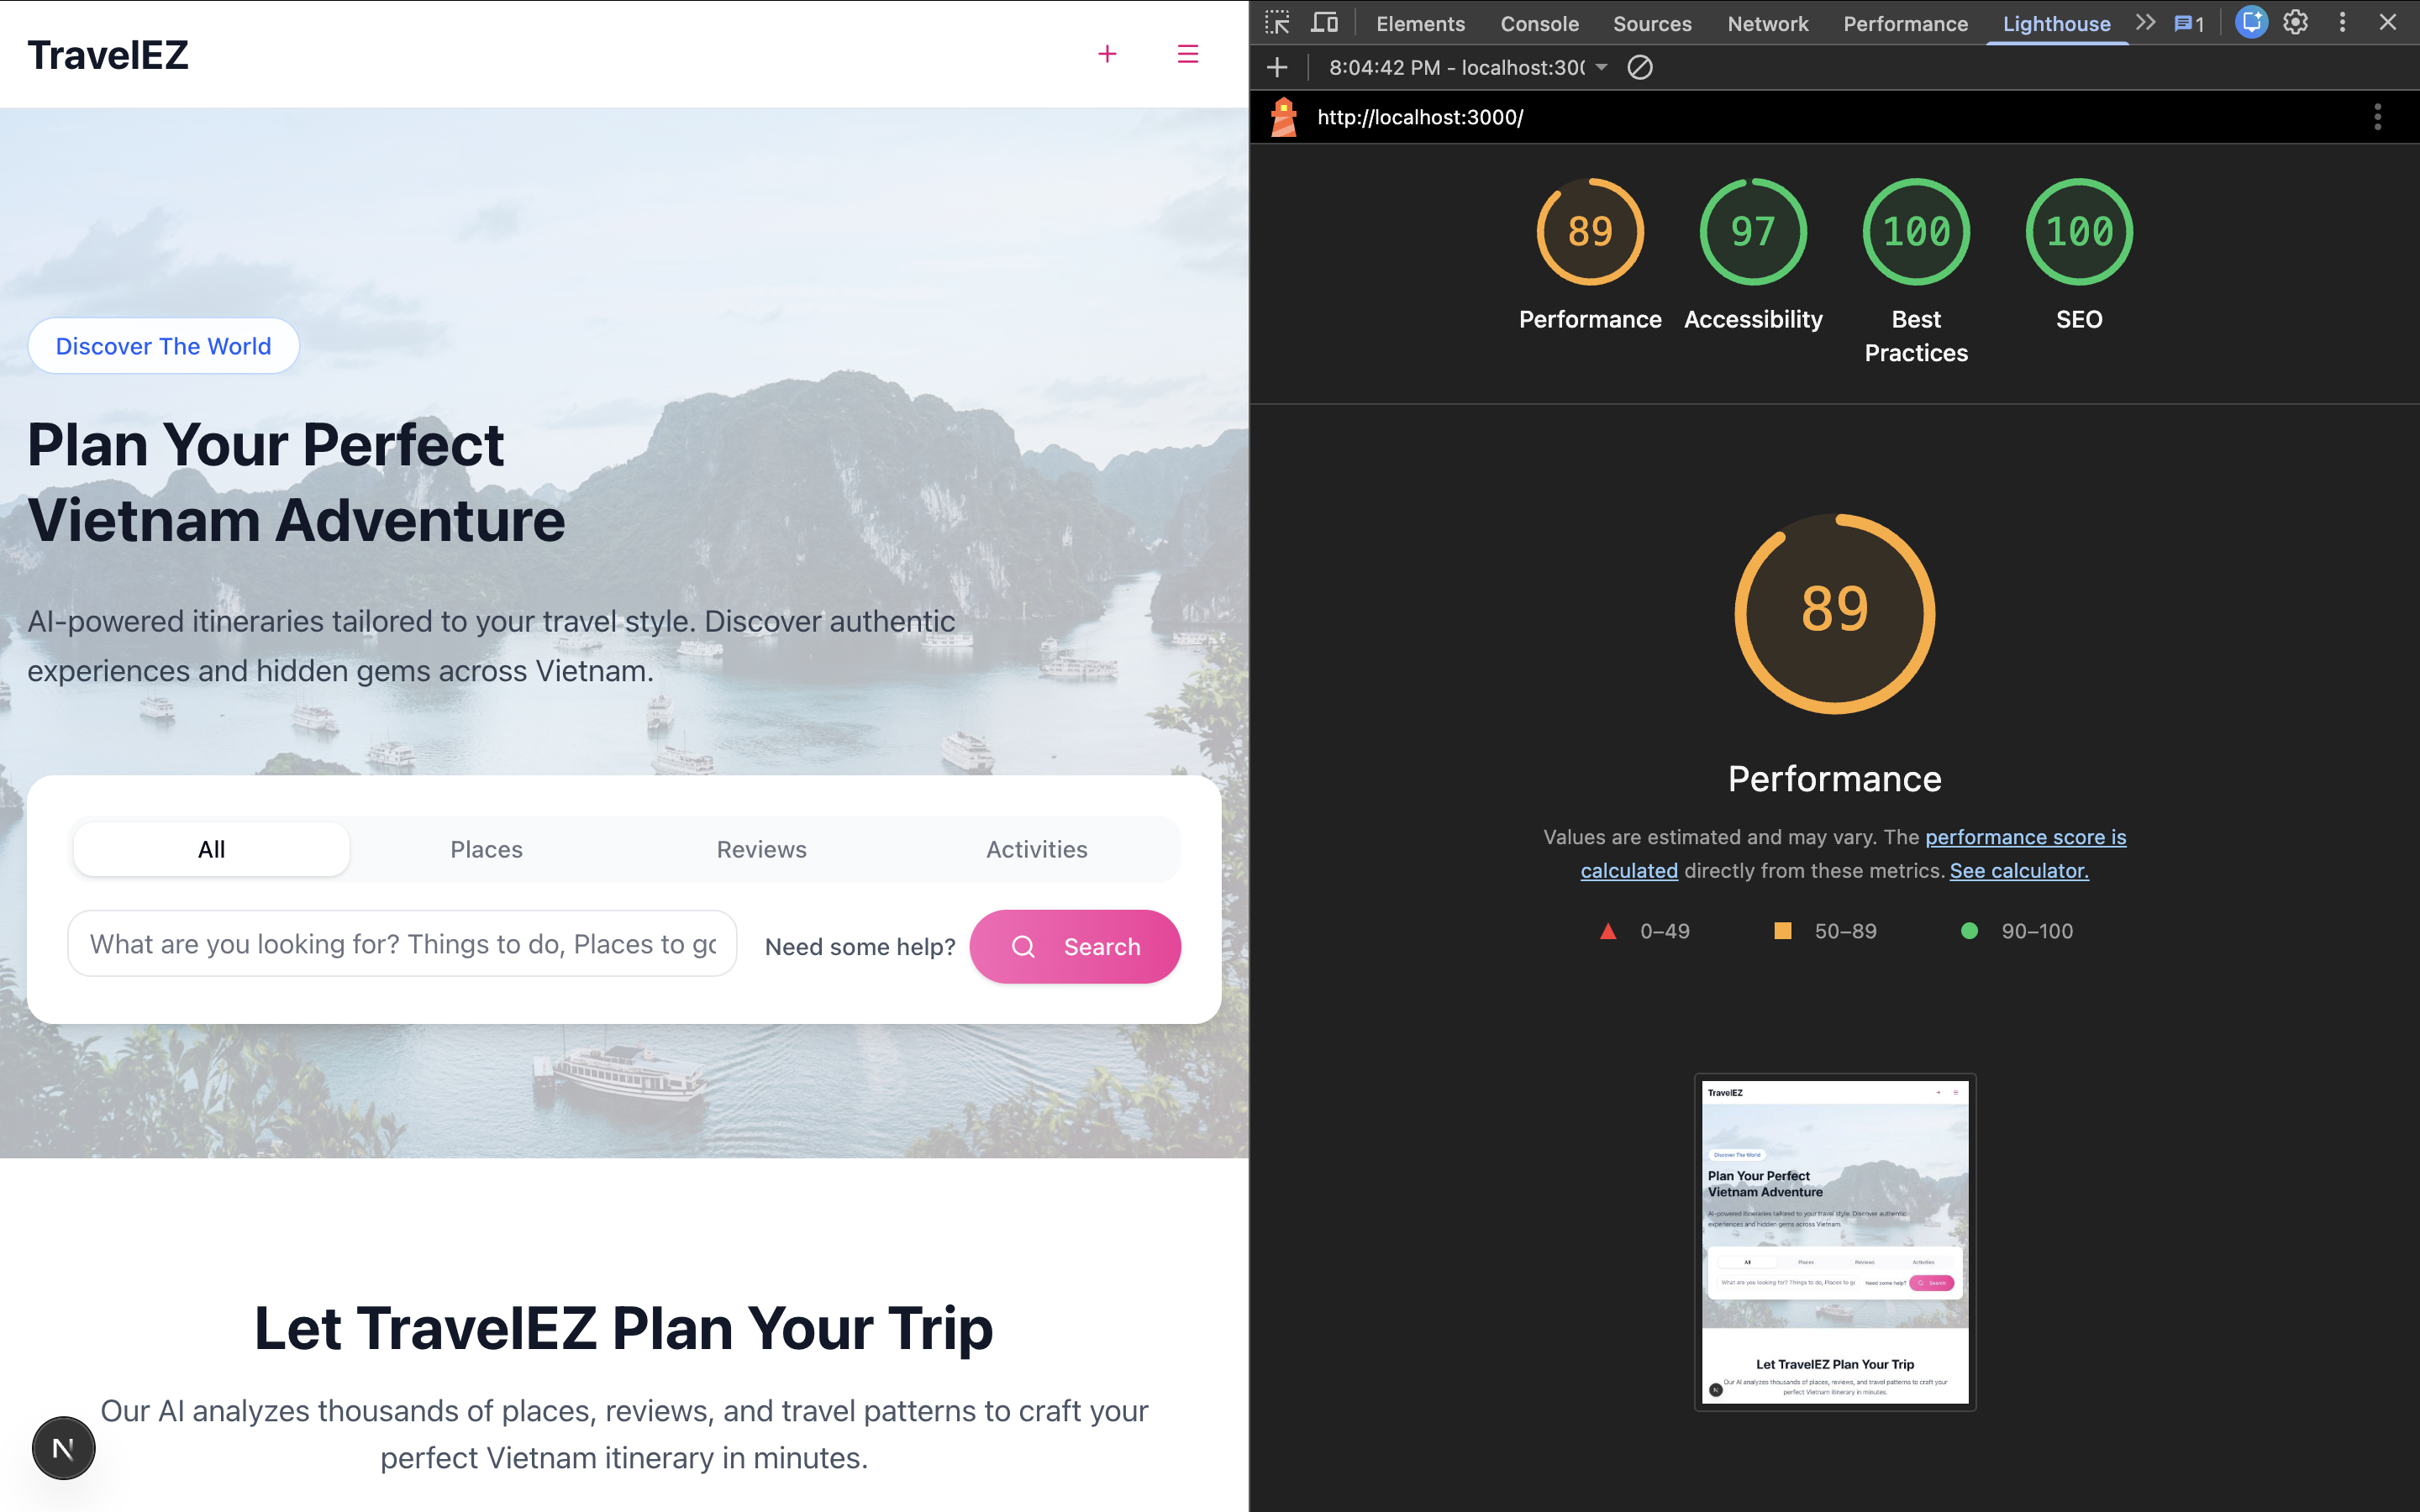
\includegraphics[width=\linewidth]{Images/8. Implement/home-desktop.png}
        \caption{Lighthouse trên Desktop}
        \label{fig:lighthouse-desktop}
    \end{minipage}\hfill
    \begin{minipage}{0.48\textwidth}
        \centering
        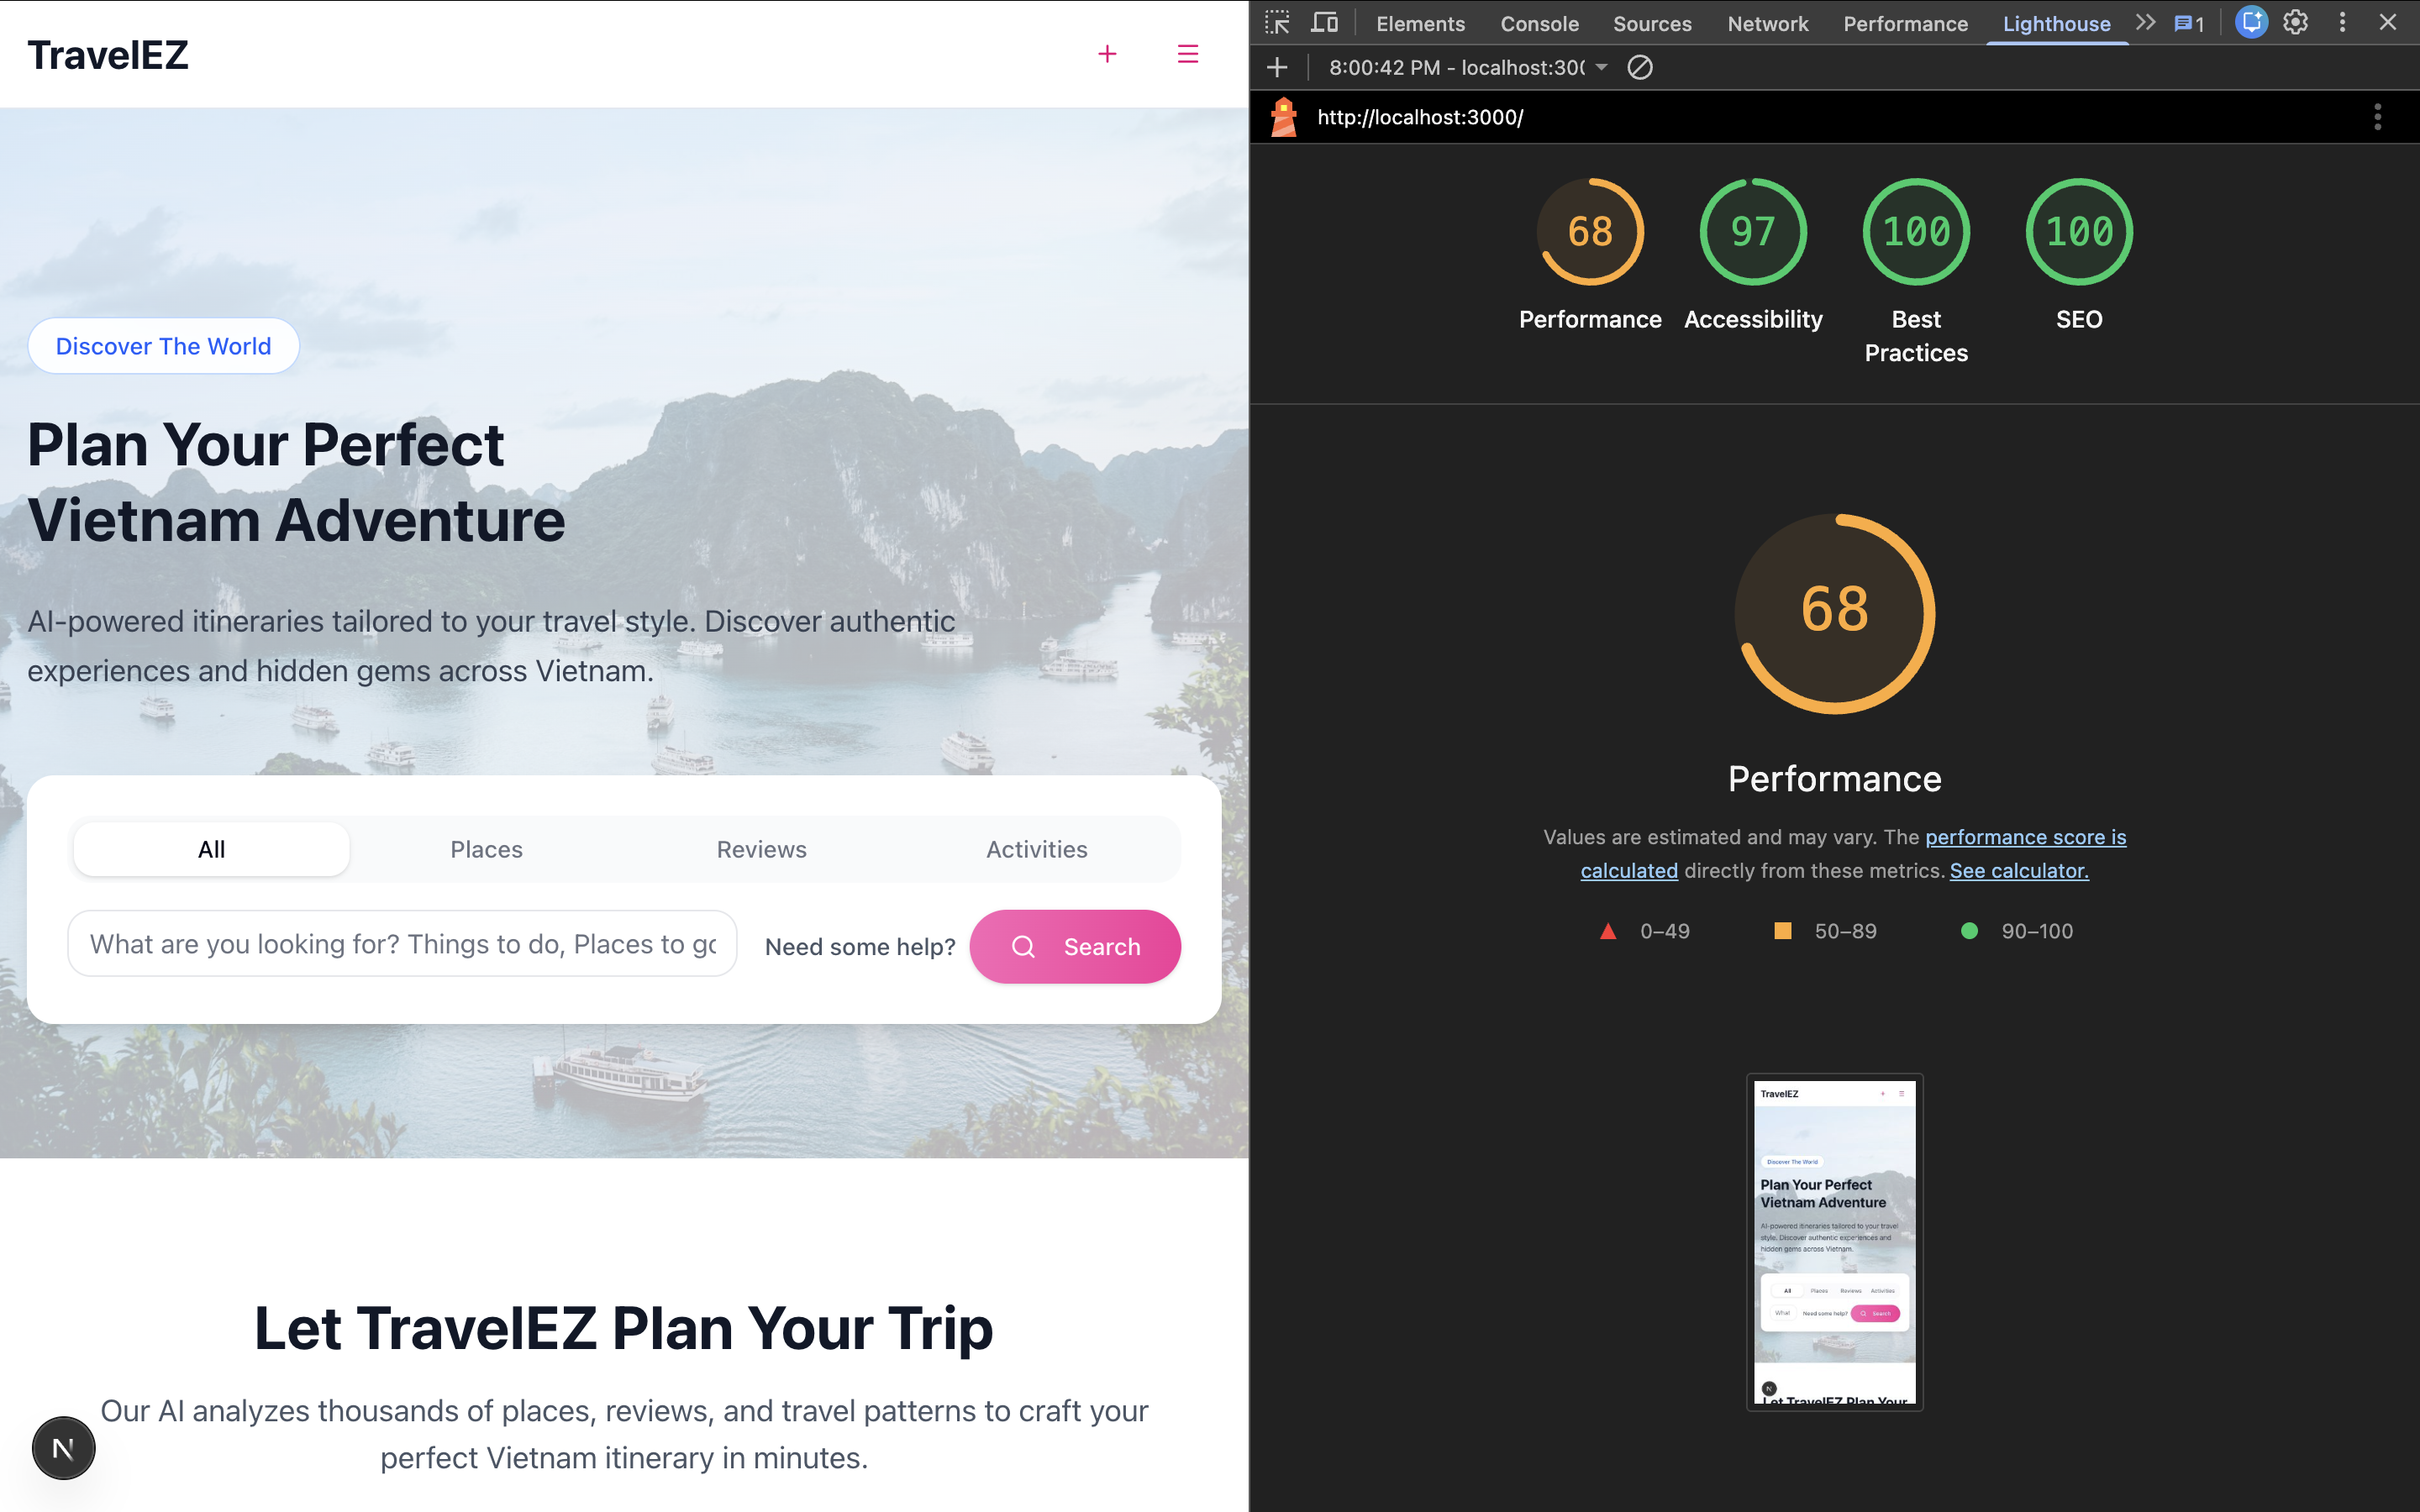
\includegraphics[width=\linewidth]{Images/8. Implement/home-mobile.png}
        \caption{Lighthouse trên Mobile}
        \label{fig:lighthouse-mobile}
    \end{minipage}
\end{figure}

\subsubsection{Thời gian tải}

Trên môi trường Desktop, ứng dụng đạt hiệu năng gần như tuyệt đối (>95 điểm), chứng minh kiến trúc Next.js hoạt động hiệu quả khi không bị giới hạn phần cứng. Trong khi đó, trên môi trường Mobile, hiệu năng giảm đáng kể (60 điểm) chủ yếu do các yếu tố bên ngoài như tốc độ mạng và giới hạn CPU. Tuy nhiên, các chỉ số về Accessibility, Best Practices và SEO vẫn duy trì ở mức cao trên cả hai nền tảng, cho thấy sự chú trọng vào chất lượng mã nguồn và trải nghiệm người dùng. 
Trong giai đoạn phát triển tiếp theo, nhóm sẽ tích hợp giải pháp Image CDN và chuyển đổi định dạng ảnh sang WebP tự động để nâng điểm số Mobile tiệm cận với Desktop.

Dựa trên kết quả biên dịch và biểu đồ thác nước (Waterfall) từ Chrome DevTools, nhóm nhận thấy một số điểm cần cải thiện để tối ưu hóa hiệu năng tải trang:
\begin{itemize}
    \item Thời gian DOM Content Loaded chỉ mất 353 ms, cho thấy cấu trúc DOM gọn nhẹ. Thời gian hoàn tất tải (Finish Load) là 1.44 s.
    \item Tổng dung lượng truyền tải là 1.4 MB. Mặc dù hơi cao so với lý thuyết, nhưng phần lớn là do hình ảnh mock data chưa tối ưu.
\end{itemize}

\begin{figure}[H]
    \centering
    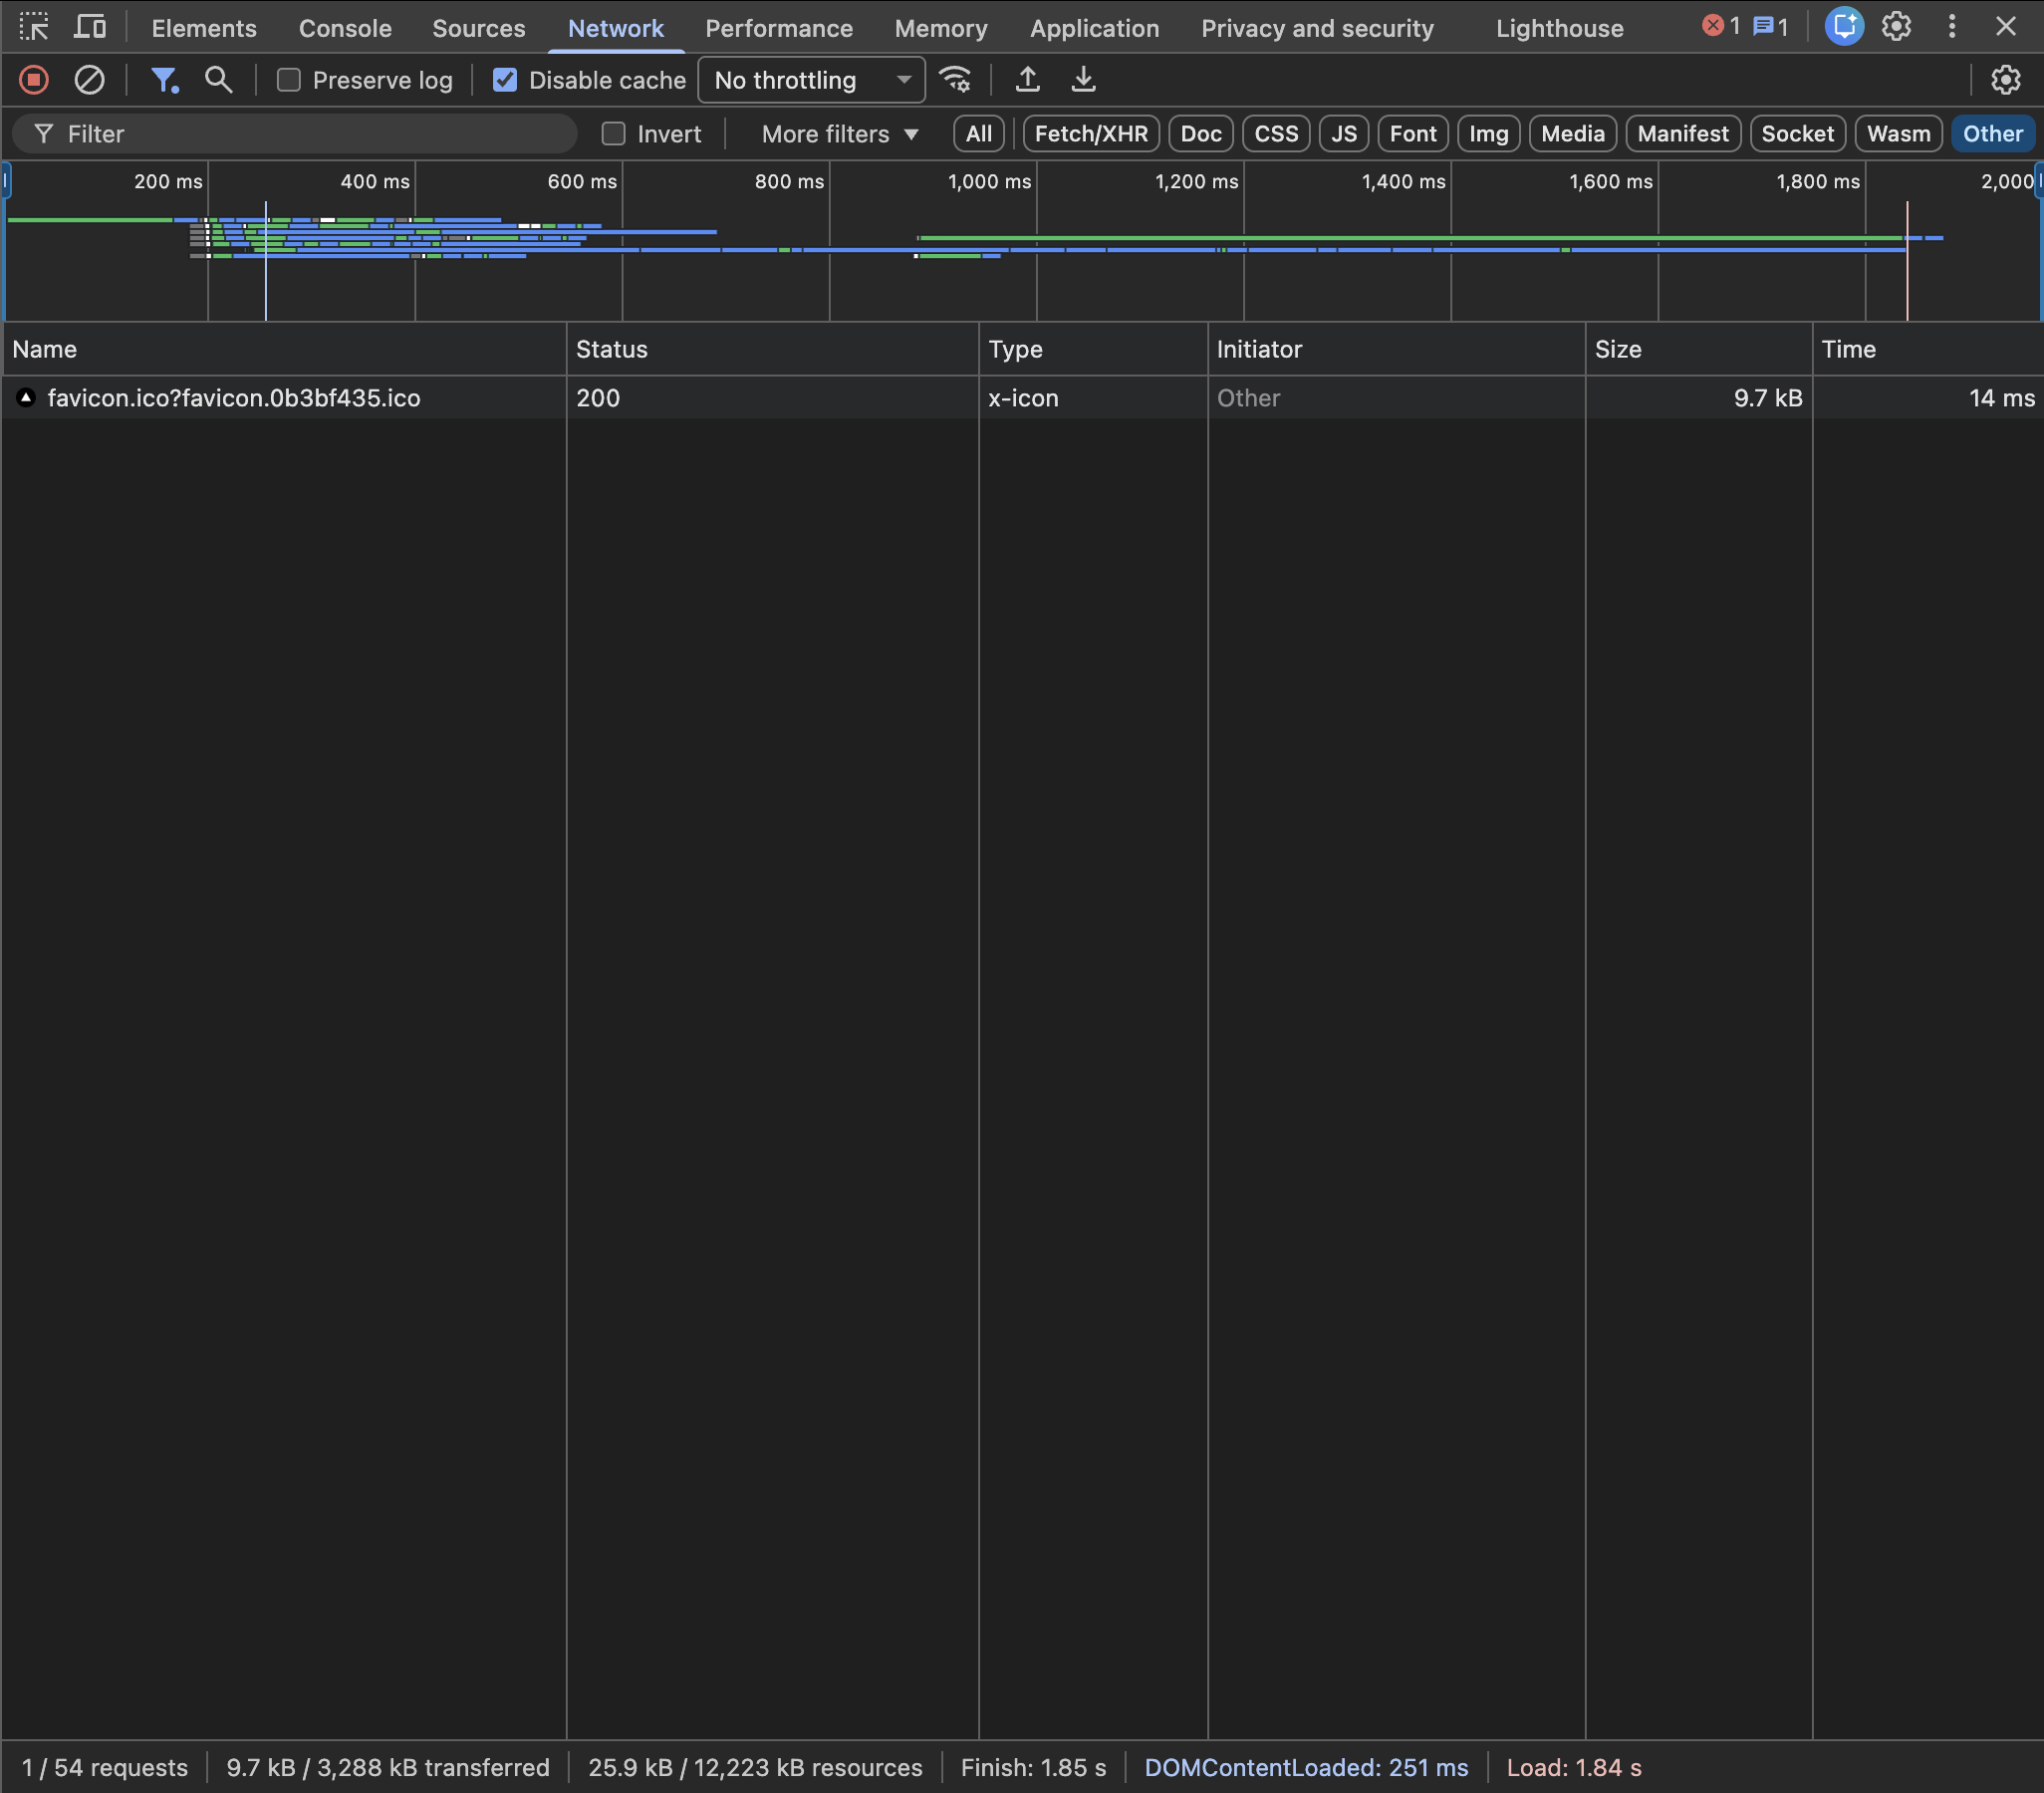
\includegraphics[width=0.8\textwidth]{Images/8. Implement/network.png}
    \caption{Kết quả biên dịch mạng từ Chrome DevTools}
    \label{fig:network}
\end{figure}

\subsubsection{Đánh giá giao diện và tương thích}
Về mặt giao diện, nhóm đã tiến hành kiểm thử trên nhiều trình duyệt Chrome. Kết quả cho thấy giao diện hiển thị đồng nhất và không gặp lỗi về bố cục hay chức năng.
\begin{itemize}
    \item Độ hoàn thiện UI: Giao diện đã được hiện thực hóa sát với bản thiết kế Figma, bao gồm các hiệu ứng chuyển động mượt mà khi chuyển đổi giữa các trang.
    \item Tính tương thích: Kiểm thử trên các viewport giả lập (iPhone 14 Pro Max, iPad Air) cho thấy layout tự động điều chỉnh linh hoạt. Các thành phần như Grid hiển thị điểm đến thay đổi từ 1 cột (Mobile) sang 3-4 cột (Desktop) mà không bị vỡ giao diện.
    \item Trạng thái hệ thống: Các tính năng tương tác như kéo thả hoạt động trơn tru trên màn hình cảm ứng, không có độ trễ đáng kể.    
\end{itemize}





